%%%%%%%%%%%%%%%%%%%%%%%%%%%%%%%%%%%%%%%%%
% kaobook
% LaTeX Template
% Version 1.0 (2/2/19)
%
% This template originates from:
% https://www.LaTeXTemplates.com
%
% Authors:
% Federico Marotta (federicomarotta@mail.com)
% Based on the doctoral thesis of Ken Arroyo Ohori (https://3d.bk.tudelft.nl/ken/en)
% and on the Tufte-LaTeX class.
% Modified for LaTeX Templates by Vel (vel@latextemplates.com)
%
% License:
% GPL Version 3 (see included LICENSE file)
%
%%%%%%%%%%%%%%%%%%%%%%%%%%%%%%%%%%%%%%%%%

%----------------------------------------------------------------------------------------
%	PACKAGES AND OTHER DOCUMENT CONFIGURATIONS
%----------------------------------------------------------------------------------------

\documentclass[
	fontsize=10pt, % Base font size
	twoside=false, % Use different layouts for even and odd pages (in particular, if twoside=true, the margin column will be always on the outside)
	%open=any, % If twoside=true, uncomment this to force new chapters to start on any page, not only on right pages
	%chapterprefix=true, % Uncomment to use the word "Chapter" before chapter numbers everywhere they appear
	%chapterentrydots=true, % Uncomment to output dots from the chapter name to the page number in the table of contents
	numbers=noenddot, % Comment to output dots after chapter numbers; the most common values for this option are: enddot, noenddot and auto (see the KOMAScript documentation for an in-depth explanation)
	%draft=true, % If uncommented, images will be replaced by empty boxes
	%overfullrule=true, % If uncommented, overly long lines will be marked by a black box
]{kaobook}

% Load common packages and commands
\usepackage{styles/environments}
\usepackage{styles/mdftheorems}
%\usepackage{styles/plaintheorems}

% Load packages for testing
\usepackage{blindtext}



\usepackage{listings}
\usepackage{color}

\definecolor{mywhite}{rgb}{0.95,0.98,1.0}
\definecolor{mygreen}{rgb}{0,0.6,0}
\definecolor{mygray}{rgb}{0.5,0.5,0.5}
\definecolor{mymauve}{rgb}{0.58,0,0.82}
% example color coding
%\iffalse
\lstset{ 
  backgroundcolor=\color{mywhite},   % choose the background color; you must add \usepackage{color} or \usepackage{xcolor}; should come as last argument
  basicstyle=\footnotesize,        % the size of the fonts that are used for the code
  breakatwhitespace=false,         % sets if automatic breaks should only happen at whitespace
  breaklines=true,                 % sets automatic line breaking
  captionpos=b,                    % sets the caption-position to bottom
  commentstyle=\color{mygreen},    % comment style
  deletekeywords={...},            % if you want to delete keywords from the given language
  escapeinside={\%*}{*)},          % if you want to add LaTeX within your code
  extendedchars=true,              % lets you use non-ASCII characters; for 8-bits encodings only, does not work with UTF-8
  %firstnumber=1000,                % start line enumeration with line 1000
  frame=single,	                   % adds a frame around the code
  keepspaces=true,                 % keeps spaces in text, useful for keeping indentation of code (possibly needs columns=flexible)
  keywordstyle=\color{blue},       % keyword style
  language=C,                 % the language of the code
  morekeywords={procedure, MoveTo, moveto, printstring, PrintString, return, Return, StartIRQ, CloseIRQ, interrupt, Procedure, ClearScreen,begin,end,loop,byte,var,program,string,integer, array,\[, \], pointer,true,false},            % if you want to add more keywords to the set
  numbers=none,                    % where to put the line-numbers; possible values are (none, left, right)
  numbersep=5pt,                   % how far the line-numbers are from the code
  numberstyle=\tiny\color{mygray}, % the style that is used for the line-numbers
  rulecolor=\color{black},         % if not set, the frame-color may be changed on line-breaks within not-black text (e.g. comments (green here))
  showspaces=false,                % show spaces everywhere adding particular underscores; it overrides 'showstringspaces'
  showstringspaces=false,          % underline spaces within strings only
  showtabs=false,                  % show tabs within strings adding particular underscores
  stepnumber=2,                    % the step between two line-numbers. If it's 1, each line will be numbered
  stringstyle=\color{mymauve},     % string literal style
  tabsize=2,	                   % sets default tabsize to 2 spaces
  title=\lstname                   % show the filename of files included with \lstinputlisting; also try caption instead of title
}



%\usepackage{fontenc}
%\usepackage[utf8]{inputenc}


%\usepackage{lmodern}
%\renewcommand{\sfdefault}{lmss}
\usepackage{lmodern}
\renewcommand*\familydefault{\sfdefault} %% Only if the base font of the document is to be sans serif
\usepackage[T1]{fontenc}
%\usepackage{showframe}
%\usepackage{showlabels}

\usepackage{courier}

\lstset{basicstyle=\footnotesize\ttfamily,breaklines=true}


\graphicspath{{images/}{./}} % Paths in which to look for images

\addbibresource{main.bib} % Bibliography file

\makeindex[columns=3, title=Alphabetical Index, intoc] % Create an index

\makeglossaries % Create a glossary

\makenomenclature % Create nomenclature

%----------------------------------------------------------------------------------------

\begin{document}

%----------------------------------------------------------------------------------------
%	BOOK INFORMATION
%----------------------------------------------------------------------------------------

\titlehead{}
\subject{A comprehensive guide to}

\title[Programming with TRSE]{Turbo Rascal Syntax Error}
\subtitle{The modern IDE and compiler for 8/16 bit computers}


\author{
	N. E. Groeneboom
	\and
	A. Hewitt 
	\and
	A. Harstad
	}

\date{\today}

\publishers{Lemonspawn Publishing AS}



%----------------------------------------------------------------------------------------

\frontmatter % Denotes the start of the pre-document content, uses roman numerals

%----------------------------------------------------------------------------------------
%	OPENING PAGE
%----------------------------------------------------------------------------------------

%\makeatletter
%\extratitle{
%	% In the title page, the title is vspaced by 9.5\baselineskip
%	\vspace*{9\baselineskip}
%	\vspace*{\parskip}
%	\begin{center}
%		% In the title page, \huge is set after the komafont for title
%		\usekomafont{title}\huge\@title
%	\end{center}
%}
%\makeatother

%----------------------------------------------------------------------------------------
%	COPYRIGHT PAGE
%----------------------------------------------------------------------------------------

\makeatletter
\uppertitleback{\@titlehead} % Header

\lowertitleback{
	\textbf{Disclaimer}\\
	You can edit this page to suit your needs. For instance, here we have a no copyright statement, a colophon and some other information. This page is based on the corresponding page of Ken Arroyo Ohori's thesis, with minimal changes.
	
	\medskip
	
	\textbf{No copyright}\\
	\cczero\ This book is released into the public domain using the CC0 code. To the extent possible under law, I waive all copyright and related or neighbouring rights to this work.
	
	To view a copy of the CC0 code, visit: \\\url{http://creativecommons.org/publicdomain/zero/1.0/}
	
	\medskip
	
	\textbf{Colophon} \\
	This document was typeset with the help of \href{https://sourceforge.net/projects/koma-script/}{\KOMAScript} and \href{ttps://www.latex-project.org/}{\LaTeX} using the \href{https://github.com/fmarotta/kaobook/}{kaobook} class.
	\medskip
	
%	\textbf{Publisher} \\
%	First printed in Jan 2019 by \@publishers
}
\makeatother

%----------------------------------------------------------------------------------------
%	DEDICATION
%----------------------------------------------------------------------------------------

\dedication{
	The best thing about a boolean is even if you are wrong, you are only off by a bit..\\
	\flushright -- Anonynous
}

%----------------------------------------------------------------------------------------
%	TITLE PAGE
%----------------------------------------------------------------------------------------

% Note that \maketitle will actually print many pages.

% If twoside=false, \uppertitleback and \lowertitleback are not printed. To overcome this issue, we set twoside=semi just before printing the title pages, and set it back to false just after the title pages.
\KOMAoptions{twoside=semi}
\maketitle[3] % The [3] assigns "page 3" to the title, so that the cover page would get "page 1" (see KOMAScript documentation about maketitle)
\KOMAoptions{twoside=false}

%----------------------------------------------------------------------------------------
%	PREFACE
%----------------------------------------------------------------------------------------

\chapter*{Preface}
\addcontentsline{toc}{chapter}{Preface}

I fondly remember playing around with my commodore 64 when I was a kid back in 1987. My father had just paid about 1500 NOK  (or about \$150) for a used specimen, which was quite a substantial amount of money in those days. He grudingly paid the price as an effort to stop my constant nagging about using his own BBC micro to play games. As I had no color screen, I was stuck using an old black \& white 12" monitor from the 1970s. 

While I primarly had an interest in playing games, I soon discovered the possibility of creating my own game using BASIC. Using the excellent Commodore 64 User's manual, I quickly learned how to make bouncing balls, small text adventures and save games to disk. However, what I never could grasp, was those pesky "POKE"s and "PEEK"s and "DATA". My 8-year old mind was just not made to understand assembly language / machine hardware at that point. For several years, I made a string of smaller text/PETSCII-based games in BASIC, but never wrote a single line of assembler. 

The Commodore 64 was slowly replaced by a successive row of IBM compatiblee PCs that I built and upgraded myself (8088, 80286 AT, 386 SX, 486 DX/2 etc), and I soon drifted into the demoscene on the PC. Here, I started to dabble in X86 assembly language, and soon discovered the excellent Turbo Pascal 5.5. My father once entered my bedroom whilst in an agitated state and threw me the user's guide for Turbo Pascal 5.5, all while saying "If you don't start learning object-oriented code, you're not my son anymore!".  While this story may or may not be entirely true, Turbo Pascal most certainly made a lasting impression on me: Combining object-oriented code (especially for 3D demo development) together with low-lever x86 assembler in a fast and efficient high-level language! During the 1990s, I created (and released) countless demoscene productions, from intros to demos and games - all made in Turbo (or Borland) Pascal.

By the late 1990s, the landscape had shifted to 32-bit protected mode programming (such as Watcom C), and I myself had shifted to dabble in those silly things that young men are prone to do - girls and beer. By the early 2000s I was working in a corporate environment writing SQL queries and using .NET. After that, I disappeared into the black hole that is University Life. However, I continued to home my programming skills by writing several Unity assets, focusing on GPU \& procedural programming, but never anything in a professional level. And no demoscene activity whatsoever. 

About two years ago (winter of 2017-2018), that all started to change. I happened to come upon The 8-bit guy's video named "The making of planet X2", a game that he had developed for the Commodore 64. I realised then that I had never actually understood anyting about the inner workings of the old breadbin - and 6502 assembly still seemed like a occult mystery to me. With renewed spirit (and perhaps some spirits), I decided to finally learn and master the basics of that old computer, a thing that had evaded me for nearly 40 years. 

After having dabbled a couple of days with 6502 assembly language (displayed an image and moved some sprites), I was completely apalled by the tediousness of maintaining assembly language code. I hadn't learned about macros, so I typed everything out. Even clearing the screen required a ton of lines, and every time I came back to the code I had to spend a long time revisiting / remembering what was going on. 

Being a very lazy guy, I decided to do what I do best: compartmentalize and hide away the details. When writing game logic, I don't want to dabble in hardware, as all the extra juggling prevents the creator to actually focus on what is important : the gameplay. There exist countless examples of technical masterpieces for these old computer systems, but very games have an advanced game logic, mostly because it is so tedious to implement in assembly language. 

A -25 degrees celsius and at remote cabin somewhere in the middle of Norway, I started developing as small C++ program called "Fluff64" that would output a C64 image (+the assembly code to display it) from a .png file. In this same program, I added support for a small text editor where you could type some simple commands such as "ClearScreen" or "PrintText". But what about parameters for these scripts? Certainly, implementing "ClearScreen(3)" or "ClearScreen(RED)" was simple enough, but what about more advanced statements such as "ClearScreen(someVariable)" or even "ClearScreen(someVariable*2+1)"? So I grabbed myself a sixpack and started going through Ruslan Spivak's excellent tutorial on "How to build an interpreter" (https://ruslanspivak.com/lsbasi-part1/). 

%Almost two years later, TRSE has become a massive beast that supports not only 


\begin{flushright}
	\textit{Nicolaas Groeneboom}
\end{flushright}


%----------------------------------------------------------------------------------------
%	TABLE OF CONTENTS & LIST OF FIGURES/TABLES
%----------------------------------------------------------------------------------------

\begingroup

% Define the style for the TOC, LOF, and LOT
%\setstretch{1}
%\hypersetup{linkcolor=DarkBlue}
\setlength{\textheight}{23cm}

% Turn on compatibility mode for the etoc package
\etocstandarddisplaystyle % "toc display" as if etoc was not loaded
\etocstandardlines % "toc lines as if etoc was not loaded

\tableofcontents % Output the table of contents

\listoffigures % Output the list of figures

% Comment both of the following lines to have the LOF and the LOT on different pages
\let\cleardoublepage\bigskip
\let\clearpage\bigskip

\listoftables % Output the list of tables

\endgroup

%----------------------------------------------------------------------------------------
%	MAIN BODY
%----------------------------------------------------------------------------------------

\mainmatter % Denotes the start of the main document content, resets page numbering and uses arabic numbers

\setchapterstyle{kao}
\setchapterpreamble[u]{\margintoc}
\chapter{Introduction}
\labch{intro}

\section{Introduction}

\begin{minipage}{0.2\textwidth}
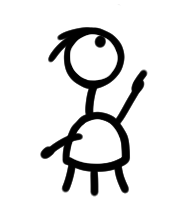
\includegraphics[width=\linewidth]{images/trip/trip1.png}
\end{minipage}
\begin{minipage}{0.8\textwidth}\raggedleft
This book serves as both a starting point and reference for anyone who is interested in learning how to develop programs using the Turbo Rascal Syntax Error ";" expected but "BEGIN" (TRSE) framework. TRSE is a modern and free IDE development for Windows, OS X and Linux that enables rapid development of software for older 8- and 16-bit systems. The ultimate goal of TRSE is to support \textbf{all} old systems, but the road is long and bumpy. Currently, TRSE supports two kinds of CPU systems: the MOS 6502 and the Motorola 68000 (or m68k).  
\end{minipage}

TRSE currently supports the following 6502 systems
\begin{itemize}
	\item Commodore 64
	\item Commodore 128 \sidenote{Not complete}
	\item VIC-20
	\item Commodore PET \sidenote{Not complete}
	\item Commodpre PLUS4 \sidenote{In development}
	\item Nintendo Entertainment System (NES) \sidenote{Not complete}
\end{itemize}
And the following Motorola 68000 systems
\begin{itemize}
	\item Amiga 500  \sidenote{Still in development}
\end{itemize}

The TRSE IDE supports several kinds of resource managements systems
\begin{itemize}
	\item Pascal editor \& parser / compiler
	\item Image and Character set (charset) editor
	\item Conversion tools
	\item Map editor
\end{itemize}


\subsection{Installation}
\label{sec:installation}
TRSE can be downloaded for free from the following location :\href{www.turborascal.com}. On Windows, no installation is required: simply extract the contents of the package to a directory and run "trse.exe". On OS X, copy the package over to the "Applications" folder.

After having installed the application, you need to specify the locations of the various emulators in the TRSE settings "emulator" panel. As emulators, we recommend using:
\begin{itemize}
	\item VICE for C64,C128,PET,VIC20 and PLUS4 emulation
	\item Mednafen for NES emulation
	\item FS-UAE for Amiga 500 emulation
\end{itemize}



\iffalse \begin{minipage}{0.8\textwidth}\raggedright
The main ideas behind kaobook come from this 
\href{https://3d.bk.tudelft.nl/ken/en/2016/04/17/a-1.5-column-layout-in-latex.html}{blog 
	post}, and actually the name of the class is dedicated to the author 
of the post, Ken Arroyo Ohori, which has kindly allowed me to create a 
class based on his thesis. Therefore, if you want to know more reasons 
to prefer a 1.5-column layout for your books, be sure to read his blog 
post.
\end{minipage}
\begin{minipage}{0.2\textwidth}
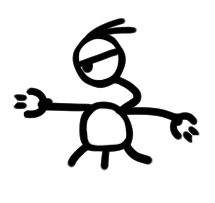
\includegraphics[width=\linewidth]{images/trip/trip2.png}
\end{minipage}

Another source of inspiration, as you may have noticed, is the 
\href{https://github.com/Tufte-LaTeX/tufte-latex}{Tufte-Latex Class}. 
The fact that the design is similar is due to the fact that it is very 
difficult to improve something wich is already so good. However, I like 
to think that this class is more flexible than Tufte-Latex. For 
instance, I have tried to use only standard packages and to implement as 
little as possible from scratch;\sidenote{This also means that 
understanding and contributing to the class development is made easier. 
Indeed, many things still need to be improved, so if you are interested, 
check out the repository on github!} therefore, it should be pretty easy 
to customise anything, provided that you read the documentation of the 
package that provides that feature.

In this book I shall illustrate the main features of the class and 
provide information about how to use and change things. Let us get 
started.

\section{What this class does}
\labsec{does}

The \Class{kaobook} class focuses more about the document structure than 
about the style. Indeed, it is a well-known \LaTeX\xspace principle that 
structure and style should be separated as much as possible (see also 
\vrefsec{doesnot}). This means that this class will only provide 
commands, environments and in general, the opportunity to do things, 
which the user may or may not use. Actually, some stylistic matters are 
embedded in the class, but the user is able to customise them with ease.

The main features are the following:

\begin{description}
	\item[Page Layout] The text width is reduced to improve readability 
	and make space for the margins, where any sort of elements can be 
	displayed.
	\item[Chapter Headings] As opposed to Tufte-Latex, we provide a 
	variety of chapter headings among which to choose; examples will be 
	seen in later chapters.
	\item[Page Headers] They span the whole page, margins included, and, 
	in twoside mode, display alternatively the chapter and the section 
	name.\sidenote[-2mm][]{This is another departure from Tufte's 
	design.}
	\item[Matters] The commands \Command{frontmatter}, 
	\Command{mainmatter} and \Command{backmatter} have been redefined in 
	order to have automatically wide margins in the main matter, and 
	narrow margins in the front and back matters. However, the page 
	style can be changed at any moment, even in the middle of the 
	document.
	\item[Margin text] We provide commands \Command{sidenote} and 
	\Command{marginnote} to put text in the 
	margins.\sidenote[-2mm][]{Sidenotes (like this!) are numbered while 
	marginnotes are not}
	\item[Margin figs/tabs] A couple of useful environments is 
	\Environment{marginfigure} and \Environment{margintable}, which, not 
	surprisingly, allow you to put figures and tables in the margins 
	(\cfr \reffig{marginmonalisa}).
	\item[Margin toc] Finally, since we have wide margins, why don't add 
	a little table of contents in them? See \Command{margintoc} for 
	that.
	\item[Hyperref] \Package{hyperref} is loaded and by default we try 
	to add bookmarks in a sensible way; in particular, the bookmarks 
	levels are automatically reset at \Command{appendix} and 
	\Command{backmatter}. Moreover, we also provide a small package to 
	ease the hyperreferencing of other parts of the text.
	\item[Bibliography] We want the reader to be able to know what has 
	been cited without having to go to the end of the document every 
	time, so citations go in the margins as well as at the end, as in 
	Tufte-Latex. Unlike that class, however, you are free to customise 
	the citations as you wish.
\end{description}

\begin{marginfigure}[-5.5cm]
	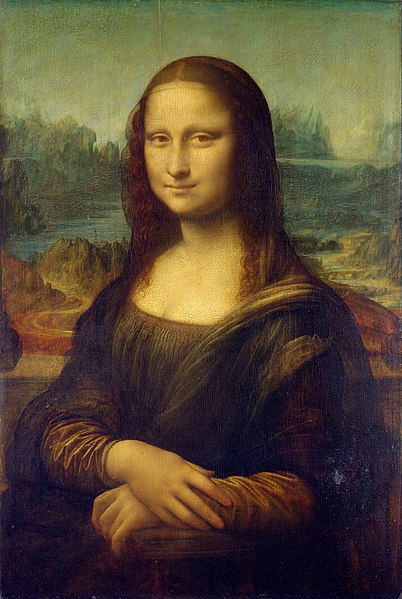
\includegraphics{monalisa}
	\caption[The Mona Lisa]{The Mona Lisa.\\ 
	\url{https://commons.wikimedia.org/wiki/File:Mona_Lisa,_by_Leonardo_da_Vinci,_from_C2RMF_retouched.jpg}}
	\labfig{marginmonalisa}
\end{marginfigure}

The order of the title pages, table of contents and preface can be 
easily changed, as in aly \LaTeX\ document. In addition, the class is 
based on \KOMAScript's \Class{scrbook}, therefore it inherits all the 
goodies of that.

\section{What this class does not}
\labsec{doesnot}

As anticipated, further customisation of the book is left to the user. 
Indeed, every book may have sidenotes, margin figures and so on, but 
each book will have its own fonts, toc style, special environments and 
so on. For this reason, in addition to the class, we provide only 
sensible defaults, but if these features are not nedded, they can be 
left out. These special packages are located in the \Path{style} 
directory, which is organised as follows:

\begin{description}
	\item[style.sty] This package contains the specifications of page 
	layout, headers and footers, chapter headings, and the fonts used 
	throughout the document.
	\item[packages.sty] Loads additional packages to decorate the 
	writing with special contents (for instance, the \Package{listing} 
	package is loaded here as it is not required in every book). There 
	are also defined some useful commands to print the same words always 
	in the same way, \eg latin words in italics or \Package{packages} in 
	verbatim.
	\item[references.sty] Some useful commands to manage labeling and 
	referencing, again to ensure that the same elements are referenced 
	always in a consistent way.
	\item[environments.sty] Provides special environments, like boxes. 
	Both simple and complex environments are available; by complex we 
	mean that they are endowed with a counter, floating and can be put 
	in a special table of contents.\sidenote[-2mm][]{See 
	\vrefch{mathematics} for some examples.}
	\item[theorems.sty] The style of mathematical environments. 
	Acutally, there are two such packages: one is for plain theorems, 
	\ie the theorems are printed in plain text; the other uses 
	\Package{mdframed} to draw a box around theorems. You can plug the 
	most appropriate style into its document.
\end{description}

\marginnote[2mm]{The audacious users might feel tempted to edit some of 
these packages. I'd be immensely happy if they sent me examples of what 
they have been able to do!}

In the rest of the book, I shall assume that the reader is not a novice 
in the use of \LaTeX, and refer to the documentation of the packages 
used in this class for things that are already explained there. 
Moreover, I assume that the reader is willing to make minor edits to the 
provided packages for styles, environments and commands, if he or she 
does not like the default settings.

\fi

\pagelayout{wide} % No margins
\addpart{Commodore 64 development}
\pagelayout{margin} % Restore margins

\setchapterstyle{kao}
\setchapterpreamble[u]{\margintoc}
\chapter{Turbo Rascal Syntax}
\labch{intro}

\section{Introcuction}

\begin{minipage}{0.2\textwidth}
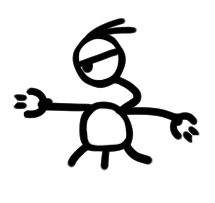
\includegraphics[width=\linewidth]{images/trip/trip2.png}
\end{minipage}
\begin{minipage}{0.8\textwidth}\raggedleft
The programming language used in TRSE is called "Rascal" for a good reason. Developed as a practical hybrid language, it is a mix of 80\% Pascal with 20\% C standards, whichever suited the developer at the time of creation. Therefore, Turbo Rascal can not be considered a fully Pascal-compliant language, since it contains some quirks. That being said, most of the syntax is definitely very Pascal-compliant indeed.   
\end{minipage}
\subsection{Program structure}
\begin{lstlisting}
Program MyProgram;
var
    a,b,c : byte = 0;
 
Procedure Myprocedure(mp_i:byte);
var
  somProcedureVariable : byte;
begin
  // Do someting
end;
 
// This is the main block.
begin
   // Call user-defined procedures etc
   MyProcedure(2);
end.
\end{lstlisting}
\subsection{Supported types}
TRSE supports several data types:
\begin{itemize}
  \item byte : values 0-255
   \item integer: values 0-65535
  \item pointer : 16 address
  \item strings are stream of bytes that are terminated with "0"
  \item incbin : include binary file
  \item incsid : include SID file
\end{itemize}
The motorola 68000 as some additional types:
\begin{itemize}
    \item long : 32 bit numbers
    \item pointer of byte/integer/long : pointer to byte/integer/long array (motorola 68000 only)
    \item chipmem specifier: myArray: array[255] of byte chipmem
\end{itemize}
Declaration examples:
\begin{lstlisting}
var
   a,b,c : byte; // will default be "0"
   d,e,f : byte = $5; // initialized with value $5
   g : integer = $1000;
   text : string = ("A STRING", 34, " CAN CONSIST OF BOTH", 45, 99, "TEXT AND NUMBERS"); // terminated by "0"
   data : incbin("data/myTable.bin", $2000); // Include data file at memory position $2000
   zp, cp : pointer; // zeropage pointers that can point to other variables / arrays
\end{lstlisting}
\subsection{Arrays}
Arrays are defined in the following manner:
\begin{lstlisting}
@define someConstant 25
 
var
   myArray1 : array[128] of byte; // 128 bytes of zeros are declared
   myArray2 : array[4*3] of byte = (0,5,$90, @someConstant);
   myArray3 : array[] of integer = ($1000, $2000, $3000); // unspecified array count
   myArray4 : array[255-55] of byte = (1,2,3); // only 3 values defined, rest will be padded with zeros.
\end{lstlisting}
Arrays that have no intialization values are filled with "0" by default. 
Arrays (both integer and bytes) are accessed as such:
\begin{lstlisting}
myArray[i]:=someValue*5;
\end{lstlisting}
There is no out-of bonds testing in TRSE.
\subsection{Conditionals}
An if-else block in TRSE is defined as such:
\subsubsection{If}
\begin{lstlisting}
if (a=1) then DoSomething();
if (a<>3) then 
begin
   DoSomethingElse();
   IgnoreMe(4);
end;
if (a*2=b*3) then 
   return() 
else
  somethingelse()
\end{lstlisting}
Do not the missing ";" before an else-block. This is a typical symptom of Pascal. 
A final note: The “empty” conditional
\begin{lstlisting}
if (a) then DoSomething() else DoSomethingElse();
\end{lstlisting}
is the same as typing “if (a<>0)” or "if (a<>true)" (if a is not true).
\subsubsection{While}
While conditionals works similar to if statements:
\begin{lstlisting}
while (a>0) then do 
begin
  PrintSomething(a);
  dec(a);
end;
\end{lstlisting}

\subsubsection{Case}
Cases tests a single variable for multiple values as such:
\begin{lstlisting}
 case i of:
   0: DoSomething();
   1: begin 
        HelloThere();
        b:=b+5;
      end;
   2+i : ThisIsWeird();
  else 
     begin
       PerformElseBlock();
     end;
\end{lstlisting}
The else block is optional.

\subsection{For loops}
For 6502 systems, only bytes are allowed as counter variables, restricting the counting loop to 256 iterations. 
\begin{lstlisting}
for i:=0 to 10 do 
begin
   doSomething(i);
end;
 
for j:=a to b step 2 do 
  someArray[j]:=a+b*j;

for j:=0 to 256 do myTable[j]:=j/16; // same as for j:=0 to 0 do ...
\end{lstlisting}
In order to overcome the 256 byte limitations, zero page pointers should be used. For instance, in order to fill the entire screen memoru at \$0400 with data, we use the following nested loop:
\begin{lstlisting}
program fillScreenWithRandomValues;
var
  x,y : byte;
  zp : pointer;

begin
	// Repeat for ever
	while (true) do
	begin

		zp:=screen_char_loc; 
		// zp now points to the screen character location (at $0400)

		// Now loop through 25 rows on the screen
		for y:=0 to 25 do 
		begin
			for x:=0 to 40 do
				zp[x]:=Random(); //Set the character with some random value

			// Increase the screen pointer by 40 bytes (width of screen)
			zp:=zp+40; 
		end;
	end;
end.
\end{lstlisting}


\subsection{Procedures}
Procedures are defined as such:
\begin{lstlisting}
Procedure NoParameters();
begin
   // .. code here
end;
 
// Procedure with single parameter and variable block
procedure DoSomething(a,b:byte; zp: pointer);
var
  localVar : byte;
 
begin
   zp:=zp+a;
   localVar := a+b; 
   // ...
end;

\end{lstlisting}
You can return byte values from procedures by using the ReturnByte(value) method. 
\begin{lstlisting}
Procedure CalculateSomeStuff(v:byte);
begin
	ReturnByte(v*2 +1);
end;

...

begin
	a:=CalculateSomeStuff(i/3)*5-1;

...
\end{lstlisting}

\subsection{Preprocessors}

\subsubsection{Constants}
\begin{lstlisting}

\end{lstlisting}

\subsubsection{Ifdef/ifndef}
\begin{lstlisting}

\end{lstlisting}

\setchapterstyle{kao}
\setchapterpreamble[u]{\margintoc}
\chapter{Introduction to C64 programming}
\labch{intro}
\section{Prerequisites}
Before you start, there are a couple of things that we need to get out of the way. In order to learn how to program for the Commodore 64 (or any other old type of computer), you need a couple of things:
\begin{itemize}
\item Some time on your hand
\item A willingless to learn
\item Basic knowledge of computer stuff
\item Having downloaded and set up Turbo Rascal SE  (\href{https://lemonspawn.com/turbo-rascal-syntax-error-expected-but-begin/turbo-rascal-se-tutorials/setup-and-introduction}), see section \ref{sec:installation}.
\end{itemize}
Having \textit{A basic knowledge of computer stuff} implies:
\begin{itemize}
\item You should know how bits and bytes, binary and hexadecimal representations work. If you don't, check out \href{https://computer.howstuffworks.com/bytes.htm} or google it. 
\item You should have an basic understanding of how programming works, ideally you know some modern programming langauges (C\#/Python) etc
\item Don't be afraid of experimenting with programs. This is how you learn: by first copying, then experiment and finally master. 
\end{itemize}
\subsection{The good \& the bad}
The \textbf{bad news} is that you will be working on an old, slow microprocessor in a programming language with absolutely no advanced stuff, no structures, no object-oriented design. If your program crashes, the computer will freeze and you will manually have to debug using a monitor. No protected mode, direct access to all hardware at any time.

\begin{minipage}{0.8\textwidth}
The \textbf{good news} is that you will be working on an old, slow microprocessor in a programming language with absolutely no advanced stuff, no structures, and no object-oriented design. You will swiflty learn how to access the hardware directly, and finally be able to understand and master almost every single piece of the computer. Not because you are exceptionally smart, but rather because the C64 is so easy to understand. As soon as you have grasped the basics. Therefore, let's start with the basics!
\end{minipage}
\begin{minipage}{0.2\textwidth}
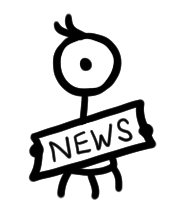
\includegraphics[width=\linewidth]{images/trip/trip11.png}
\end{minipage}

\section{The Commodore 64}
The Commodore 64 uses a MOS technologies 8-bit 6510 microprocessor (a variant of the 6502) clocked in at 0.985 MHz (PAL version). It has a 16 bit address register allowing for $2^16 = 65535 = \$FFFF = 64kb$ of memory, but actually has a bit more than this when ROM (read-only-memory) is included. The "GPU" (graphics chip) of the C64 is called the Video Interface Chip (VIC), and shares the same RAM/ROM as the C64. This means that the data feeding the signal that the VIC chip is producing is directly accessible by the CPU.

When the computer starts up, the VIC screen points to memory address \$0400. When you run a TRSE program, the default memory location for the program is at \$800, but the BASIC is overloaded and told to execute your program (starting at \$810) instead. Let's create a TRSE program that changes a byte on the screen:
\subsection{My First Program}
\begin{lstlisting}
program MostBasicProgram;
begin
	poke(^$0400,0,1);
	Loop();
end.
\end{lstlisting}

\begin{minipage}{0.2\textwidth}
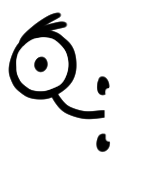
\includegraphics[width=\linewidth]{images/trip/trip12.png}
\end{minipage}
\begin{minipage}{0.8\textwidth}
"Poke" means "Set byte at memory address". Poke(\^\$0400,0,1) therefore translates to "Set the value of memory address \$0400+0 to be "1". Then loop the program ad infinitum. Incidentally, \$0400 is the beginning of screen space, and therefore represents the character in the upper-left corner of the screen. Value "1" corresponds to the ROM screen character for "A".
\end{minipage}

\begin{minipage}{0.8\textwidth}
The VIC addressing is somewhat skewed, since it can only access 16kb of ram. This means that the VIC address space is evenly divided into 4 "banks" on the c64: from \$0000-\$3FFF, \$4000-\$7FFF, \$8000-\$BFFF and finally \$C000-\$FFFF. When you tell the VIC chip to "use bank 2", what you are doing is telling it to access and use memory from \$8000-\$BFFF.
\end{minipage}
\begin{minipage}{0.2\textwidth}
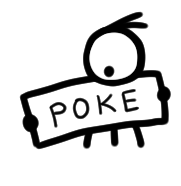
\includegraphics[width=\linewidth]{images/trip/trip7.png}
\end{minipage}


\section{TRSE Tutorials}
\subsection{Hello World}
\begin{minipage}{0.8\textwidth}
\begin{lstlisting}
program HelloWorld;
var  
  	text : string = ("HELLO WORLD");

begin
	// Fill the screen (at screen_char_loc) with character $20 - "space"
	ClearScreen($20, screen_char_loc);
	// Fill the color ram with yellow
	ClearScreen(yellow, screen_col_loc);
	// Move cursor to x,y position 10,12
	moveto(10,12,$04);
	// Print the text
	printstring(text,0,40);
	// Move cursor 2 rows down (2*40)
	screenmemory:=screenmemory+2*40;
	// Print something else
	printstring("THIS IS ANOTHER STRING",0,40);
	// Infinite loop
	Loop(); 
end.
\end{lstlisting}
\end{minipage}
\begin{minipage}{0.2\textwidth}
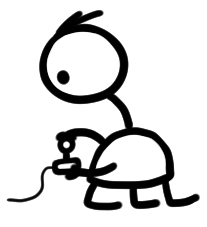
\includegraphics[width=\linewidth]{images/trip/trip8.png}
\end{minipage}

\begin{minipage}{0.6\textwidth}
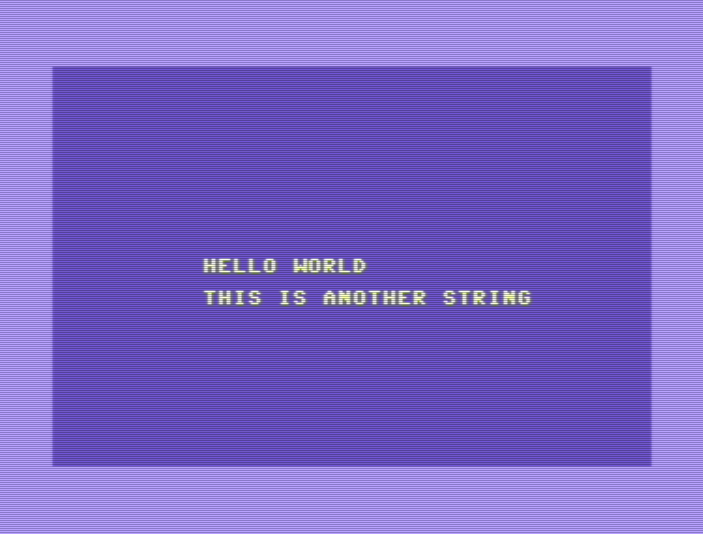
\includegraphics{images/c64/01_helloworld.png}
\end{minipage}
\begin{minipage}{0.4\textwidth}
Lorem ipsum dolor sit amet, quo ex molestiae philosophia. Qui periculis sententiae comprehensam eu, audiam accusamus consequat eum no, no nam legimus placerat. Qui no dictas accusamus, no vim liberavisse instructior. Ius quaeque utroque tincidunt ei, his saperet consequat eu.
\end{minipage}
Te autem impetus ius, vel facer omnes mediocrem in. Timeam persius eligendi at sed, eu vitae noster latine vel. Liberavisse definitiones comprehensam te sea. Pri ne mollis expetenda, cum habeo quaestio maiestatis an. Ne vim senserit sapientem dissentiet. Et vis ceteros lucilius, ad aperiri argumentum vis.


\subsection{Texty}
\begin{minipage}{0.8\textwidth}
\begin{lstlisting}
program Texty;
var  
	// Define three variables : position x, position y and time
   x,y,time,i: byte = 0;  
begin
 	// First, fill color ram with white
	ClearScreen(white, screen_col_loc);
	// Set black border
	screen_bg_col:=black;
	// infinite loop
	while (true) do
	begin
		// Make sure we wait for 1 raster cycle to complete
		waitforraster(0);
		// Clear screen with character $20 (space)
		ClearScreen($20, screen_char_loc);
		// Calculate x,y some sine values (making a circle)
		// if sine[x] then sine[x+64] is equal to cosine  
		x:=sine[time]/12 + 6;		
		y:=sine[time+64]/16 + 4;		
		// move "screenmemory" cursor to x,y at screen memory $0400
		moveto(x,y,$04);
		
		i:=time/64; // i will now have values between 0 and 3 (since time is between 0 and 255)
		// Print some random string
		case i of
			0:	printstring("I AM FISH",0,40);
			1:	printstring("ARE YOU FISH",0,40);
			2:	printstring("ME AM CAT",0,40);
			3:	printstring("OM NOM NOM",0,40);
		end;
		// Increase the timer
		time:=time+1;
	end;

end.
\end{lstlisting}
\end{minipage}
\begin{minipage}{0.2\textwidth}
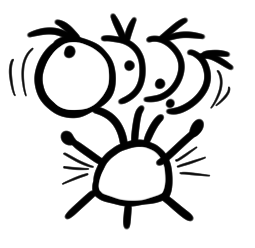
\includegraphics[width=\linewidth]{images/trip/trip9.png}
\end{minipage}

\begin{minipage}{0.4\textwidth}
Lorem ipsum dolor sit amet, quo ex molestiae philosophia. Qui periculis sententiae comprehensam eu, audiam accusamus consequat eum no, no nam legimus placerat. Qui no dictas accusamus, no vim liberavisse instructior. Ius quaeque utroque tincidunt ei, his saperet consequat eu.
\end{minipage}
\begin{minipage}{0.6\textwidth}
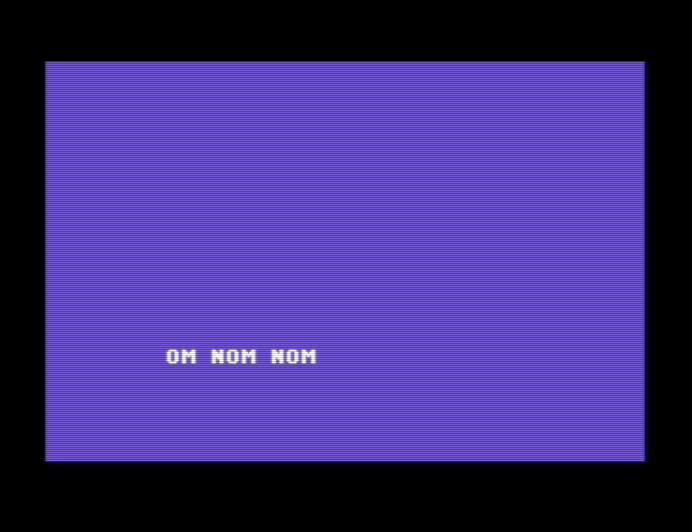
\includegraphics{images/c64/02_texty.png}
\end{minipage}
Te autem impetus ius, vel facer omnes mediocrem in. Timeam persius eligendi at sed, eu vitae noster latine vel. Liberavisse definitiones comprehensam te sea. Pri ne mollis expetenda, cum habeo quaestio maiestatis an. Ne vim senserit sapientem dissentiet. Et vis ceteros lucilius, ad aperiri argumentum vis.


\subsection{Boxes}
\begin{minipage}{0.8\textwidth}
\begin{lstlisting}
program Boxes;
var  
	saddr: array[25] of integer; // Screen address table
	caddr: array[25] of integer; // Color adress table
	
	box: array[8] of byte = ($55, $43, $49, $5d, $4b, $43, $4a, $5d);
	x,y,dx,dy,t: byte = 0;

	
begin
	// Set screen background/border color
	screen_bg_col:=black;
	screen_fg_col:=black;
	
    clearscreen($20, screen_char_loc);
    clearscreen(black, screen_col_loc);
	// Sets up the address tables for the screen & color memory    
	createaddresstable(saddr,screen_char_loc,40,25);
	createaddresstable(caddr,screen_col_loc,40,25);

	// dx and dy are initialized to 1
	dx:=1;
	dy:=1;
	while (true) do begin
		// Make sure we only draw 1 box per frame
		waitforraster(80);
		// Add the delta dx and dy to x and y
		x:=x+dx;
		y:=y+dy;
		// Flip dx and dy when borders are reached
	    case x of
		    	31: dx := -1;
		    	0: dx := 1;
		end;
	    case y of
	    		20: dy := -1;
	    		0: dy := 1;
		end;
		// Make sure that t loops from 0-15
		t:=(t+1)&15;
		// Draw two boxes in opposing corners
		drawcolortextbox(saddr, caddr, box, x, y, 9, 5, t);
		drawcolortextbox(saddr, caddr, box, 31 - x, 20 - y, 9, 5, 16 - t);
	end;
end.\end{lstlisting}
\end{minipage}
\begin{minipage}{0.2\textwidth}
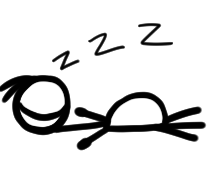
\includegraphics[width=\linewidth]{images/trip/trip10.png}
\end{minipage}

\begin{minipage}{0.4\textwidth}
Lorem ipsum dolor sit amet, quo ex molestiae philosophia. Qui periculis sententiae comprehensam eu, audiam accusamus consequat eum no, no nam legimus placerat. Qui no dictas accusamus, no vim liberavisse instructior. Ius quaeque utroque tincidunt ei, his saperet consequat eu.
\end{minipage}
\begin{minipage}{0.6\textwidth}
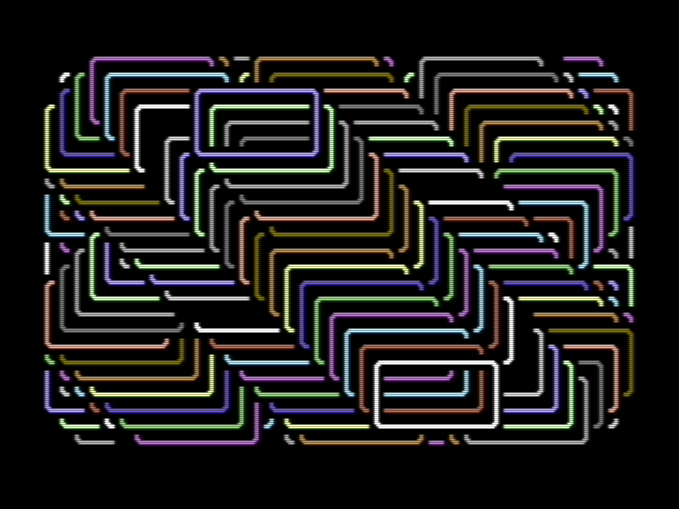
\includegraphics{images/c64/03_boxes.png}
\end{minipage}
Te autem impetus ius, vel facer omnes mediocrem in. Timeam persius eligendi at sed, eu vitae noster latine vel. Liberavisse definitiones comprehensam te sea. Pri ne mollis expetenda, cum habeo quaestio maiestatis an. Ne vim senserit sapientem dissentiet. Et vis ceteros lucilius, ad aperiri argumentum vis.


\subsection{Randomness ahoy!}
\begin{lstlisting}
program Randomness;
var  
	random_color,x,y,index: byte; 
	// Array of random bytes
	random_values : array[256] of byte; 
	// Pointer to screen and color ram
	screenP, colorP : pointer;



// Initialize a random table of 256 bytes
// generator
procedure InitializeRandom();
begin
	// same as : for x:=0 to 0 do begin..
	for x:=0 to 256 do begin 
		random_values[x]:=Random();
    end;
end;

begin
	InitializeRandom();
	// Set screen foreground and background to black. The second parameter is an offset.
	screen_bg_col:=black;
	screen_fg_col:=black;
	
	// point to start of random table
	index:=0; 
	// infinite loop
	while (true) do  begin
		// Set pointer to point to beginning of screen/color ram ($0400 and $D800)
		screenP:=screen_char_loc;
		colorP:=screen_col_loc;
		// loop y		
		for y:=0 to 24 do begin
			// moves current screen position
			// Select some random color
			for x:=0 to 40 do begin
				// Sets both screen and color values
				screenP[x] := random_values[index];
				// increases screen X counter
				// Increase by some random non-repeatable prime
				index:=index+17;
	    		end;
			// Select some random color
			random_color := random_values[index];
			// Fill the current line in colorP with 40 bytes of random_color
			fill(colorP,random_color,40);
			// Increase screen and color pointers
			screenP:=screenP+40;
			colorP:=colorP+40;
			end
	end;

end.
\end{lstlisting}

\begin{minipage}{0.4\textwidth}
Lorem ipsum dolor sit amet, quo ex molestiae philosophia. Qui periculis sententiae comprehensam eu, audiam accusamus consequat eum no, no nam legimus placerat. Qui no dictas accusamus, no vim liberavisse instructior. Ius quaeque utroque tincidunt ei, his saperet consequat eu.
\end{minipage}
\begin{minipage}{0.6\textwidth}
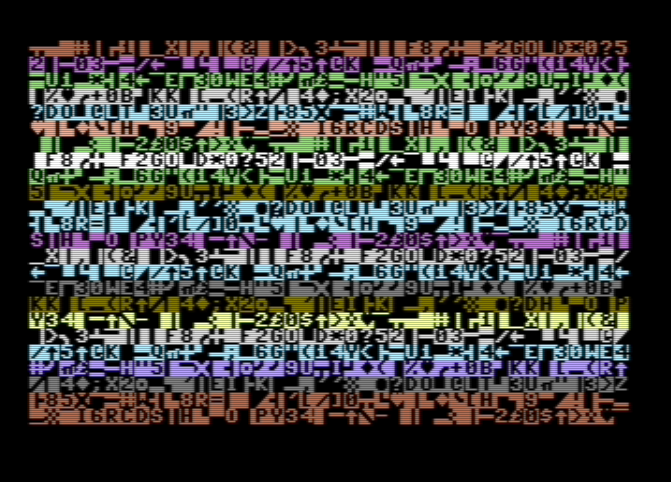
\includegraphics{images/c64/04_randomness.png}
\end{minipage}
Te autem impetus ius, vel facer omnes mediocrem in. Timeam persius eligendi at sed, eu vitae noster latine vel. Liberavisse definitiones comprehensam te sea. Pri ne mollis expetenda, cum habeo quaestio maiestatis an. Ne vim senserit sapientem dissentiet. Et vis ceteros lucilius, ad aperiri argumentum vis.


\subsection{Plasma}
Definitions and arrays.
\\
\begin{minipage}{0.8\textwidth}
\begin{lstlisting}
program Tutorial3_plasma;

var
	// some plasma variables
	c,val,c2x, c2y,ax, ay : byte;
	x,y : byte;
	colorP: pointer;	

// charset will be placed at $2000 in bank 1	
@define charsetLocation $2000
 // look in the character set
@define baseCharacter $68

	// Use custom charset
	charset: IncBin("charsets/charset.bin",@charsetLocation);
	// nice colors
	fade : array [] of byte = (11,6,12,12,4,14,15,1,1,1,1,15,14,4,12,12,6,11,1,1); 
	

	// mini sine table
    siny : array[25] of byte; 
	sinx : array[40] of byte; 

	// Lookup table for division by 16
	lookupDiv16 : array[256] of byte;


// Define y_start as a global preprocessor constant
@define y_start "5"
\end{lstlisting}
\end{minipage}
\begin{minipage}{0.2\textwidth}
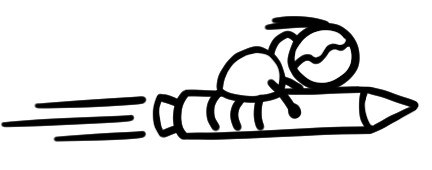
\includegraphics[width=\linewidth]{images/trip/trip13.png}
\end{minipage}

The plasma method itself!\\

\begin{minipage}{0.8\textwidth}
\begin{lstlisting}
procedure Plasma();
begin
	c2x:=ax;
	c2y:=ay;
	
	// Set up y-sine table
	for x:=0 to 25 do begin 
		siny[x]:=  sine[c2x] + sine[c2y];
		c2x:=c2x+4;
		c2y:=c2y+9;
	end;

	ax:=ax+3;
	ay:=ay-5;

	// Set up x-sine table
	for x:=0 to 40 do begin 
		sinx[x] := sine[c2x] + sine[c2y];
		c2x:=c2x+3;
		c2y:=c2y+7;

	end;
	// Move cursor to (1,y) on $0400 on bank 1
	moveto(1,@y_start, $04);
	// moveto could also be replaced with : screenmemory:=$0400 + @y_start*40;
	
	colorP:=screen_col_loc + @y_start*40;
	
	for y:=@y_start to 23 do begin
		val:=siny[y];
		for x:=1 to 36 do begin
			// here, we take (sin[x]+val) and divide by 16. However, since this is a slow procedure,
			// we have created a lookup table instead!
			c:=lookupDiv16[ (sinx[x] +val) ];
			// Set the screen memory
			screenmemory[x]:=c + @baseCharacter;
			// Set color memory
			colorP[x] := fade[ c ];

		end;
		// Increase screen memory pointer by 40 (next row)
		screenmemory:=screenmemory+40;
		// Increase color pointer by 40 (next row)
		colorP:=colorP+40;
	end;

end;
\end{lstlisting}
\end{minipage}

\begin{minipage}{0.2\textwidth}
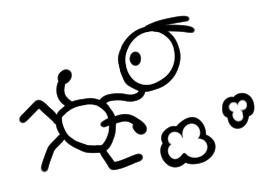
\includegraphics[width=\linewidth]{images/trip/trip14.png}
\end{minipage}


The main method\\
\begin{minipage}{0.8\textwidth}
\begin{lstlisting}
procedure InitDivision16();
begin
	for x:=0 to 256 do lookupDiv16[x]:=x/16; // Simply store values divided by 16
end;

begin
	// Set color background
	screen_bg_col:=black;
	screen_fg_col:=black;
	// Set charmap location at $2000
	SetCharsetLocation(@charsetLocation);
	InitDivision16();
	ax:=1;
	ay:=5;

	// Clear screen and color memory
	ClearScreen($20, screen_char_loc);
	// Main loop
	while (true) do begin
		waitForRaster(0);
		Plasma();
	end;
end.
\end{lstlisting}
\end{minipage}
\begin{minipage}{0.2\textwidth}
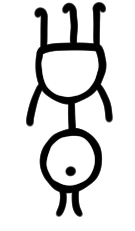
\includegraphics[width=\linewidth]{images/trip/trip15.png}
\end{minipage}




\begin{minipage}{0.6\textwidth}
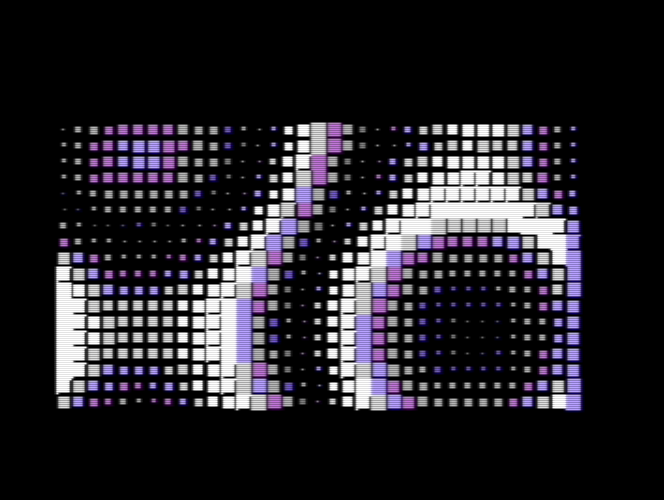
\includegraphics{images/c64/06_plasma.png}
\end{minipage}
\begin{minipage}{0.4\textwidth}
Lorem ipsum dolor sit amet, quo ex molestiae philosophia. Qui periculis sententiae comprehensam eu, audiam accusamus consequat eum no, no nam legimus placerat. Qui no dictas accusamus, no vim liberavisse instructior. Ius quaeque utroque tincidunt ei, his saperet consequat eu.
\end{minipage}
Te autem impetus ius, vel facer omnes mediocrem in. Timeam persius eligendi at sed, eu vitae noster latine vel. Liberavisse definitiones comprehensam te sea. Pri ne mollis expetenda, cum habeo quaestio maiestatis an. Ne vim senserit sapientem dissentiet. Et vis ceteros lucilius, ad aperiri argumentum vis.


\section{What's an interrupt?}
Imagine you are painting your apartement - in the 20th floor. Since you have to be finished by tomorrow, you have asked three of your friends to come help you. But the problem is that you don't know exactly when each of them will show up. 
\\
Now, why is it a problem that you don't know exactly when they show up you may wonder? The door bell on the 1st floor is broken. So you constantly have to run down from the 20th floor, open the door, check for friends, run back up, paint 30 seconds, run down again to the 1st floor, open the door, check for friends, run back up, paint 30 seconds, run do..... ok! You get the point. The only thing you will be busy with is waiting. Ideally, you would like to start painting your apartement and just be INTERRUPTED when each of your friends ring the door bell. But since this interrupt mechanism is broken, you need to find another solution: the mobile phone.
\\
So, instead you call your friends and tell them to use their mobile phones to ring you when they are downstairs. In that way you can constantly keep painting, and be notified (INTERRUPTED) only when you friends are ready downstairs.
\\
What's this story do to with programming the C64 with TRSE? Well, of course this was just an analogy. But if we want to make smart and effective programs we need to have the 6510 CPU work at full speed - with real tasks - and only be interrupted when something important happens! And when the interrupt routine is completed the CPU goes back to the tasks it was interrupted from.
\\
Ok, let's gets started! 
\\
\subsection{Avoiding busy waits - our first simple interrupt routine}
In the story above you see that it is possible to constantly run up and down to check for you friends, but it's not very effective. The same goes for the C64 - you can have the CPU to just sit and wait for something to happen (BUSY WAIT).  

Let's look at an example. Below you find a small program that set the background color to black at line 0, and turn it to yellow at line 150. Copy and paste this sample into TRSE and run it!
\begin{lstlisting}
program BusyWait;
var

procedure MainLoop();
begin
	WaitForRaster(0);
	SCREEN_BG_COL:=BLACK;
	
	WaitForRaster(150);
	SCREEN_BG_COL:=YELLOW;
end;

begin
	while(0<1) then begin
		MainLoop();
	end;
end.
\end{lstlisting}What is the problem with this program? It's switching from black to yellow? Well, the function WaitForRaster() prevents the CPU of doing anything else while waiting. In a real program you would like to do a lot of stuff while waiting for a rasterline such as calculating new sprite positions, moving a scrolltext, preparing a new screen in a different videobank etc. 

Now, how would this program look if we would like to use interrupts instead? It would look like this: 
\begin{lstlisting}
program RasterInterrupt;
var  
	@define useKernal 0
	
interrupt InterruptRoutine02();

interrupt InterruptRoutine01();
begin
	StartIRQ(@useKernal);
	SCREEN_BG_COL:=BLACK;

	RasterIRQ(InterruptRoutine02(),150,@useKernal);
	
	CloseIRQ();
end;

interrupt InterruptRoutine02();
begin
	StartIRQ(@useKernal);
	SCREEN_BG_COL:=YELLOW;

	RasterIRQ(InterruptRoutine01(),0,@useKernal);
	
	CloseIRQ();
end;

procedure MainLoop();
begin
	// Insert your program here
end;


begin
	preventirq();
	disableciainterrupts();
	setmemoryconfig(1,@useKernal,0);
	enablerasterirq();
	rasterirq(InterruptRoutine01(),0,@useKernal);
	enableirq();

	while (0<1) then begin
		MainLoop();
	end;
end.
\end{lstlisting}
First of all note this: the MainLoop() does NOTHING now! This means that you are now free to do anything you like in the MainLoop, and the background will still be colored black and yellow! The interrupts does this for you! 

Lets's go trough the program and explain everything step-by-step!








busy waits
different types of interrupts
needs to be masked






broken = masked

Types of interrupts on the C64 (NMI, BRK, CIA, VICs)

KERNAL vs HW

Basics of interrupts

	- Trigger
	- Interrupt routine
	- Acknowledge
	- Return

Sample - VIC raster interrupt



%\input{chapters/textnotes.tex}
%\input{chapters/figsntabs.tex}
%\ProvidesPackage{styles/references}

% Easily label and reference elements
% Note that \label must appear after \caption
% hyperref is already loaded
\usepackage{varioref}
%\usepackage{cleveref} % Don't use cleveref! It breaks everything
\newcommand{\sectionname}{Section}

\newcommand{\labpage}[1]{\label{page:#1}}
\newcommand{\labpart}[1]{\label{part:#1}}
\newcommand{\labch}[1]{\label{ch:#1}}
\newcommand{\labsec}[1]{\label{sec:#1}}
\newcommand{\labfig}[1]{\label{fig:#1}}
\newcommand{\labtab}[1]{\label{tab:#1}}
\newcommand{\labdef}[1]{\label{def:#1}}
\newcommand{\labthm}[1]{\label{thm:#1}}
\newcommand{\labprop}[1]{\label{prop:#1}}
\newcommand{\lablemma}[1]{\label{lemma:#1}}
\newcommand{\labremark}[1]{\label{remark:#1}}
\newcommand{\labexample}[1]{\label{example:#1}}
\newcommand{\labexercise}[1]{\label{exercise:#1}}

\newcommand{\refpage}[1]{\hyperref[#1]{Page}~\pageref{page:#1}} % Page 84
\newcommand{\vrefpage}[1]{\vpageref*{page:#1}} % on the following page, on page 84

\newcommand{\refpart}[1]{\hyperref[part:#1]{Part}~\ref{part:#1}} % Part IV
\newcommand{\vrefpart}[1]{\hyperref[part:#1]{Part}~\vref{part:#1}} % Part IV, Part IV on the following page, Part IV on page 84
\newcommand{\nrefpart}[1]{\hyperref[part:#1]{Part}~\ref{part:#1} (\nameref{part:#1})}
\newcommand{\frefpart}[1]{\hyperref[part:#1]{Part~\ref{part:#1} (\nameref{part:#1}) \vpageref{part{#1}}}} % Part IV (Name of the Part), Part IV (Name of the Part) on the following page, Part IV (Name of the Part) on page 84)

%\newcommand{\refch}[1]{\hyperref[#1]{\chaptername~\usekomafont{chapter}\normalsize\nameref{ch:#1}}\xspace\vpageref{ch:#1}\,}
\newcommand{\refch}[1]{\hyperref[ch:#1]{\chaptername~\ref{ch:#1}}}
\newcommand{\vrefch}[1]{\hyperref[ch:#1]{\chaptername~\vref{ch:#1}}}
\newcommand{\nrefch}[1]{\hyperref[ch:#1]{\chaptername~\ref{ch:#1} (\nameref{ch:#1})}}
\newcommand{\frefch}[1]{\hyperref[ch:#1]{\chaptername~\ref{ch:#1} (\nameref{ch:#1}) \vpageref{ch:#1}}}

%\newcommand{\refsec}[1]{Section~{\usekomafont{section}\normalsize\nameref{sec:#1}}\xspace\vpageref{sec:#1}\,}
\newcommand{\refsec}[1]{\hyperref[sec:#1]{\sectionname~\ref{sec:#1}}}
\newcommand{\vrefsec}[1]{\hyperref[sec:#1]{\sectionname~\vref{sec:#1}}}
\newcommand{\nrefsec}[1]{\hyperref[sec:#1]{\sectionname~\ref{sec:#1} (\nameref{sec:#1})}}
\newcommand{\frefsec}[1]{\hyperref[sec:#1]{\sectionname~\ref{sec:#1} (\nameref{sec:#1}) \vpageref{sec:#1}}}

%\newcommand{\reffig}[1]{{\hypersetup{colorlinks=false}\usekomafont{captionlabel}\hyperref[fig:#1]{Figure}\xspace\ref{fig:#1}}}
\newcommand{\reffig}[1]{\hyperref[fig:#1]{Figure}\xspace\ref{fig:#1}}
\newcommand{\vreffig}[1]{\hyperref[fig:#1]{Figure\xspace\vref{fig:#1}}}

%\newcommand{\reftab}[1]{{\hypersetup{colorlinks=false}\usekomafont{captionlabel}\hyperref[tab:#1]{Table}\xspace\ref{tab:#1}}}
\newcommand{\reftab}[1]{\hyperref[tab:#1]{Table}\xspace\ref{tab:#1}}
\newcommand{\vreftab}[1]{\hyperref[tab:#1]{Table\xspace\vref{tab:#1}}}

\newcommand{\refdef}[1]{\hyperref[def:#1]{Definition}\xspace\ref{def:#1}}
\newcommand{\vrefdef}[1]{\hyperref[def:#1]{Definition}\xspace\vref{def:#1}}

\newcommand{\refthm}[1]{\hyperref[thm:#1]{Theorem}\xspace\ref{thm:#1}}
\newcommand{\vrefthm}[1]{\hyperref[thm:#1]{Theorem}\xspace\vref{thm:#1}}

\newcommand{\refprop}[1]{\hyperref[prop:#1]{Proposition}\xspace\ref{prop:#1}}
\newcommand{\vrefprop}[1]{\hyperref[prop:#1]{Proposition}\xspace\vref{prop:#1}}

\newcommand{\reflemma}[1]{\hyperref[lemma:#1]{Lemma}\xspace\ref{lemma:#1}}
\newcommand{\vreflemma}[1]{\hyperref[lemma:#1]{Lemma}\xspace\vref{lemma:#1}}

\newcommand{\refremark}[1]{\hyperref[remark:#1]{Remark}\xspace\ref{remark:#1}}
\newcommand{\vrefremark}[1]{\hyperref[remark:#1]{Remark}\xspace\vref{remark:#1}}

\newcommand{\refexample}[1]{\hyperref[example:#1]{Example}\xspace\ref{example:#1}}
\newcommand{\vrefexample}[1]{\hyperref[example:#1]{Example}\xspace\vref{example:#1}}

\newcommand{\refexercise}[1]{\hyperref[exercise:#1]{Exercise}\xspace\ref{exercise:#1}}
\newcommand{\vrefexercise}[1]{\hyperref[exercise:#1]{Exercise}\xspace\vref{exercise:#1}}


%\pagelayout{wide} % No margins
%\addpart{Design and Additional Features}
%\pagelayout{margin} % Restore margins

%\input{chapters/layout.tex}
%\input{chapters/mathematics.tex}

\appendix % From here onwards, chapters are numbered with letters, as is the appendix convention

\pagelayout{wide} % No margins
\addpart{Appendix}
\pagelayout{margin} % Restore margins

\setchapterstyle{lines}
\labpage{appendix}
\section{TRSE methods and constants}
\subsection{Methods}
\subsection{Constants}
\section{Commodore 64}
\subsection{Memory map}
\begin{figure}[h]
\centering
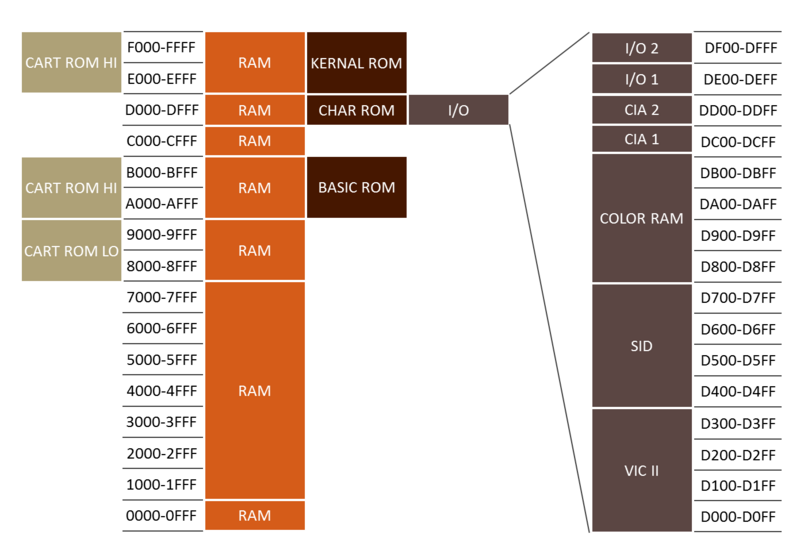
\includegraphics[width=15cm]{images/c64/memory_map.png}
\caption{The C64 memory map. From \href{https://www.c64-wiki.com}}
\end{figure}
\section{VIC-20}


%----------------------------------------------------------------------------------------

\backmatter % Denotes the end of the main document content

\setchapterstyle{plain} % Output plain chapters from this point onwards

%----------------------------------------------------------------------------------------
%	BIBLIOGRAPHY
%----------------------------------------------------------------------------------------

% The bibliography needs to be compiled on the command line with 'biber main' from the template directory

\defbibnote{bibnote}{Here are the references in citation order.\par\bigskip} % Prepend this text to the bibliography
\printbibliography[heading=bibintoc, title=Bibliography, prenote=bibnote] % Add the bibliography heading to the ToC and set the title of the bibliography

%----------------------------------------------------------------------------------------
%	NOMENCLATURE
%----------------------------------------------------------------------------------------

% The nomenclature needs to be compiled on the command line with 'makeindex main.nlo -s nomencl.ist -o main.nls' from the template directory

%\nomenclature{$c$}{Speed of light in a vacuum inertial frame}
%\nomenclature{$h$}{Planck constant}

\renewcommand{\nomname}{Notation}
\renewcommand{\nompreamble}{The next list describes several symbols that will be later used within the body of the document.}
%\printnomenclature % Output the nomenclature

%----------------------------------------------------------------------------------------
%	GREEK ALPHABET
% 	Originally from https://gitlab.com/jim.hefferon/linear-algebra
%----------------------------------------------------------------------------------------
\iffalse
\vspace{3cm}
{\usekomafont{chapter}Greek letters with pronounciation} \\[2ex]
\begin{center}
	\newcommand{\pronounced}[1]{\hspace*{.2em}\small\textit{#1}}
	\begin{tabular}{l l @{\hspace*{3em}} l l}
		\toprule
		Character & Name & Character & Name \\ 
		\midrule
		$\alpha$ & alpha \pronounced{AL-fuh} & $\nu$ & nu \pronounced{NEW} \\
		$\beta$ & beta \pronounced{BAY-tuh} & $\xi$, $\Xi$ & xi \pronounced{KSIGH} \\ 
		$\gamma$, $\Gamma$ & gamma \pronounced{GAM-muh} & o & omicron \pronounced{OM-uh-CRON} \\
		$\delta$, $\Delta$ & delta \pronounced{DEL-tuh} & $\pi$, $\Pi$ & pi \pronounced{PIE} \\
		$\epsilon$ & epsilon \pronounced{EP-suh-lon} & $\rho$ & rho \pronounced{ROW} \\
		$\zeta$ & zeta \pronounced{ZAY-tuh} & $\sigma$, $\Sigma$ & sigma \pronounced{SIG-muh} \\
		$\eta$ & eta \pronounced{AY-tuh} & $\tau$ & tau \pronounced{TOW (as in cow)} \\
		$\theta$, $\Theta$ & theta \pronounced{THAY-tuh} & $\upsilon$, $\Upsilon$ & upsilon \pronounced{OOP-suh-LON} \\
		$\iota$ & iota \pronounced{eye-OH-tuh} & $\phi$, $\Phi$ & phi \pronounced{FEE, or FI (as in hi)} \\
		$\kappa$ & kappa \pronounced{KAP-uh} & $\chi$ & chi \pronounced{KI (as in hi)} \\
		$\lambda$, $\Lambda$ & lambda \pronounced{LAM-duh} & $\psi$, $\Psi$ & psi \pronounced{SIGH, or PSIGH} \\
		$\mu$ & mu \pronounced{MEW} & $\omega$, $\Omega$ & omega \pronounced{oh-MAY-guh} \\
		\bottomrule
	\end{tabular} \\[1.5ex]
	Capitals shown are the ones that differ from Roman capitals.
\end{center}
\fi
%----------------------------------------------------------------------------------------
%	GLOSSARY
%----------------------------------------------------------------------------------------

% The glossary needs to be compiled on the command line with 'makeglossaries main' from the template directory

\newglossaryentry{computer}{
	name=computer,
	description={is a programmable machine that receives input, stores and manipulates data, and provides output in a useful format}
}

\newacronym[longplural={Frames per Second}]{fpsLabel}{FPS}{Frame per Second}
\newacronym[longplural={Tables of Contents}]{tocLabel}{TOC}{Table of Contents}

\setglossarystyle{listgroup} % Set the style of the glossary (see https://en.wikibooks.org/wiki/LaTeX/Glossary for a reference)
\printglossary[title=Special Terms, toctitle=List of terms] % Output the glossary, 'title'  is the chapter heading for the glossary, toctitle is the table of contents heading

%----------------------------------------------------------------------------------------
%	INDEX
%----------------------------------------------------------------------------------------

% The index needs to be compiled on the command line with 'makeindex main' from the template directory

\printindex % Output the index

%----------------------------------------------------------------------------------------
%	BACK COVER
%----------------------------------------------------------------------------------------

% If you have a PDF file that you want to use as back cover, uncomment the following lines.

%\clearpage
%\thispagestyle{empty}
%\null%
%\clearpage
%\includepdf{cover-back.pdf}

%----------------------------------------------------------------------------------------

\end{document}
